% python3 code_to_tex.py nyc25.py nyc25_tex && xelatex </dev/null spork_nyc25.tex
\documentclass[12pt]{article}

\usepackage[a5paper, landscape, margin=10mm]{geometry}
\usepackage{enumitem}
\usepackage{amsmath}
\usepackage{amssymb}
\usepackage{amsfonts}
\usepackage{placeins}
\usepackage{graphicx}
\usepackage{listings}
\usepackage{caption}
\usepackage{colortbl}
\usepackage[parfill]{parskip}
\usepackage[mathscr]{euscript}
\usepackage[usenames,dvipsnames,svgnames,table,hyperref]{xcolor}
\usepackage[hidelinks]{hyperref}
\usepackage{fontspec}
\usepackage{mdframed}

\setsansfont{FreeSans}
\setmonofont{Ubuntu Mono}
\renewcommand{\familydefault}{\sfdefault}

\hyphenation{WebGL}

\definecolor{webColor}{RGB}{0, 108, 174}
\newcommand{\web}[1]{{\color{webColor} \small \url{#1}}}
\newcommand{\webText}[2]{{\color{webColor} \href{#2}{#1}}}
\newcommand{\email}[2]{{\small \color{webColor} \textsf{\href{mailto:#1@#2}{#1[at]#2}}}}
\definecolor{titleColor}{RGB}{179, 0, 149}
\newcommand{\myTitle}[1]{{\large \color{titleColor} \hspace{-4mm} \textbf{\textsf{#1}}}}
\definecolor{subColor}{RGB}{179, 0, 149}
\newcommand{\mySub}[1]{\textsf{\color{subColor}#1}}
\definecolor{keyColor}{RGB}{170, 149, 0}
\newcommand{\myKey}[1]{\textbf{\color{keyColor}#1}}

\definecolor{redBoxFg}{RGB}{255, 0, 0}
\definecolor{redBoxBg}{RGB}{255, 218, 232}
\newcommand{\redBox}[1]{{\color{redBoxFg}\colorbox{redBoxBg}{#1}}}
\definecolor{yellowBoxFg}{RGB}{0, 0, 0}
\definecolor{yellowBoxBg}{RGB}{255, 232, 0}
\newcommand{\yellowBox}[1]{{\color{yellowBoxFg}\colorbox{yellowBoxBg}{#1}}}
\definecolor{greenBoxFg}{RGB}{0, 0, 0}
\definecolor{greenBoxBg}{RGB}{134, 210, 153}
\newcommand{\greenBox}[1]{{\color{greenBoxFg}\colorbox{greenBoxBg}{#1}}}
\definecolor{blueBoxFg}{RGB}{0, 0, 255}
\definecolor{blueBoxBg}{RGB}{218, 232, 255}
\newcommand{\blueBox}[1]{{\color{blueBoxFg}\colorbox{blueBoxBg}{#1}}}
\definecolor{violetBoxFg}{RGB}{0, 0, 0}
\definecolor{violetBoxBg}{RGB}{218, 204, 255}
\newcommand{\violetBox}[1]{{\color{violetBoxFg}\colorbox{violetBoxBg}{#1}}}

\mdfdefinestyle{MyFrame}{%
    linecolor=black,
    outerlinewidth=0pt,
    linewidth=0pt,
    innertopmargin=2.7pt,
    innerbottommargin=0pt,
    innerrightmargin=0pt,
    innerleftmargin=0pt,
        leftmargin = 0pt,
        rightmargin = 0pt}

\definecolor{lightttColor}{RGB}{69, 69, 80}
\newcommand{\lighttt}[1]{{\color{lightttColor}\texttt{#1}}}

\renewcommand*\labelenumi{(\theenumi)}
\renewcommand*{\theenumii}{\roman{enumii}}
\renewcommand*\labelenumii{\theenumii.}

\newcommand{\fixminipage}{\raggedright \setlength{\parskip}{0.3\baselineskip}}
\newcommand{\codeminipage}{\raggedright \setlength{\parskip}{0\baselineskip}}
\sloppy
\pagenumbering{gobble}


\begin{document}

\tikzstyle{smallnode} = [rectangle, minimum width=1.25cm, minimum height=1cm, text centered, text width=1.25cm, draw=black, fill=white]
\tikzstyle{smallishnode} = [rectangle, minimum width=2cm, minimum height=1cm, text centered, text width=2cm, draw=black, fill=white]
\tikzstyle{normalnode} = [rectangle, minimum width=3cm, minimum height=1cm, text centered, text width=3cm, draw=black, fill=white]
\tikzstyle{widenode} = [rectangle, minimum width=62mm, minimum height=8mm, text centered, text width=62mm, draw=black, fill=white]
\tikzstyle{bignode} = [rectangle, minimum width=3.5cm, minimum height=2cm, text centered, text width=3cm, draw=black, fill=white]
\tikzstyle{smemnode} = [rectangle, minimum width=3cm, minimum height=1cm, text centered, text width=3cm, draw=keyColorB, fill=white]
\tikzstyle{gmemnode} = [rectangle, minimum width=3cm, minimum height=1cm, text centered, text width=3cm, draw=keyColorA, fill=white]
\tikzstyle{smallishsmemnode} = [rectangle, minimum width=2cm, minimum height=1cm, text centered, text width=2cm, draw=keyColorB, fill=white]
\tikzstyle{arrow} = [thick,->,>=stealth]
\tikzstyle{line} = [thick]

\tikzstyle{rednode} = [normalnode, draw=redBoxFg, fill=redBoxBg, text=redBoxFg]
\tikzstyle{yellownode} = [normalnode, draw=yellowBoxFg, fill=yellowBoxBg, text=yellowBoxFg]
\tikzstyle{greennode} = [normalnode, draw=greenBoxFg, fill=greenBoxBg, text=greenBoxFg]
\tikzstyle{bluenode} = [normalnode, draw=blueBoxFg, fill=blueBoxBg, text=blueBoxFg]
\tikzstyle{violetnode} = [normalnode, draw=violetBoxFg, fill=violetBoxBg, text=violetBoxFg]

\tikzstyle{Mnode} = [greennode, text width=55mm, minimum width=55mm, minimum height=7mm]
\tikzstyle{Nnode} = [violetnode, text width=7mm, minimum width=7mm, minimum height=7mm]

\tikzstyle{producer} = [yellownode, text width=64mm, minimum width=64mm, minimum height=14mm]
\tikzstyle{consumer} = [greennode, text width=20mm, minimum width=20mm, minimum height=14mm]
\tikzstyle{smallproducer} = [yellownode, text width=20mm, minimum width=20mm, minimum height=14mm]
\tikzstyle{copylatency} = [violetnode, text width=84mm, minimum width=84mm, minimum height=8mm]
\tikzstyle{ring} = [violetnode, text width=16mm, minimum width=1mm, minimum height=14mm]
\newcommand{\consumerBox}[1]{{\color{greenBoxFg}\colorbox{greenBoxBg}{#1}}}
\newcommand{\producerBox}[1]{{\color{yellowBoxFg}\colorbox{yellowBoxBg}{#1}}}

\myBiggerTitle{Exo-GPU}

\textbf{\hfill \large Safe, Imperative, User-schedulable Programming for Tensor Cores}

{\LARGE

\vfill

David Zhao Akeley

Yuka Ikarashi

Jonathan Ragan-Kelley

\hfill \myBiggerTitle{2025 MIT/Jane Street Symposium}}

%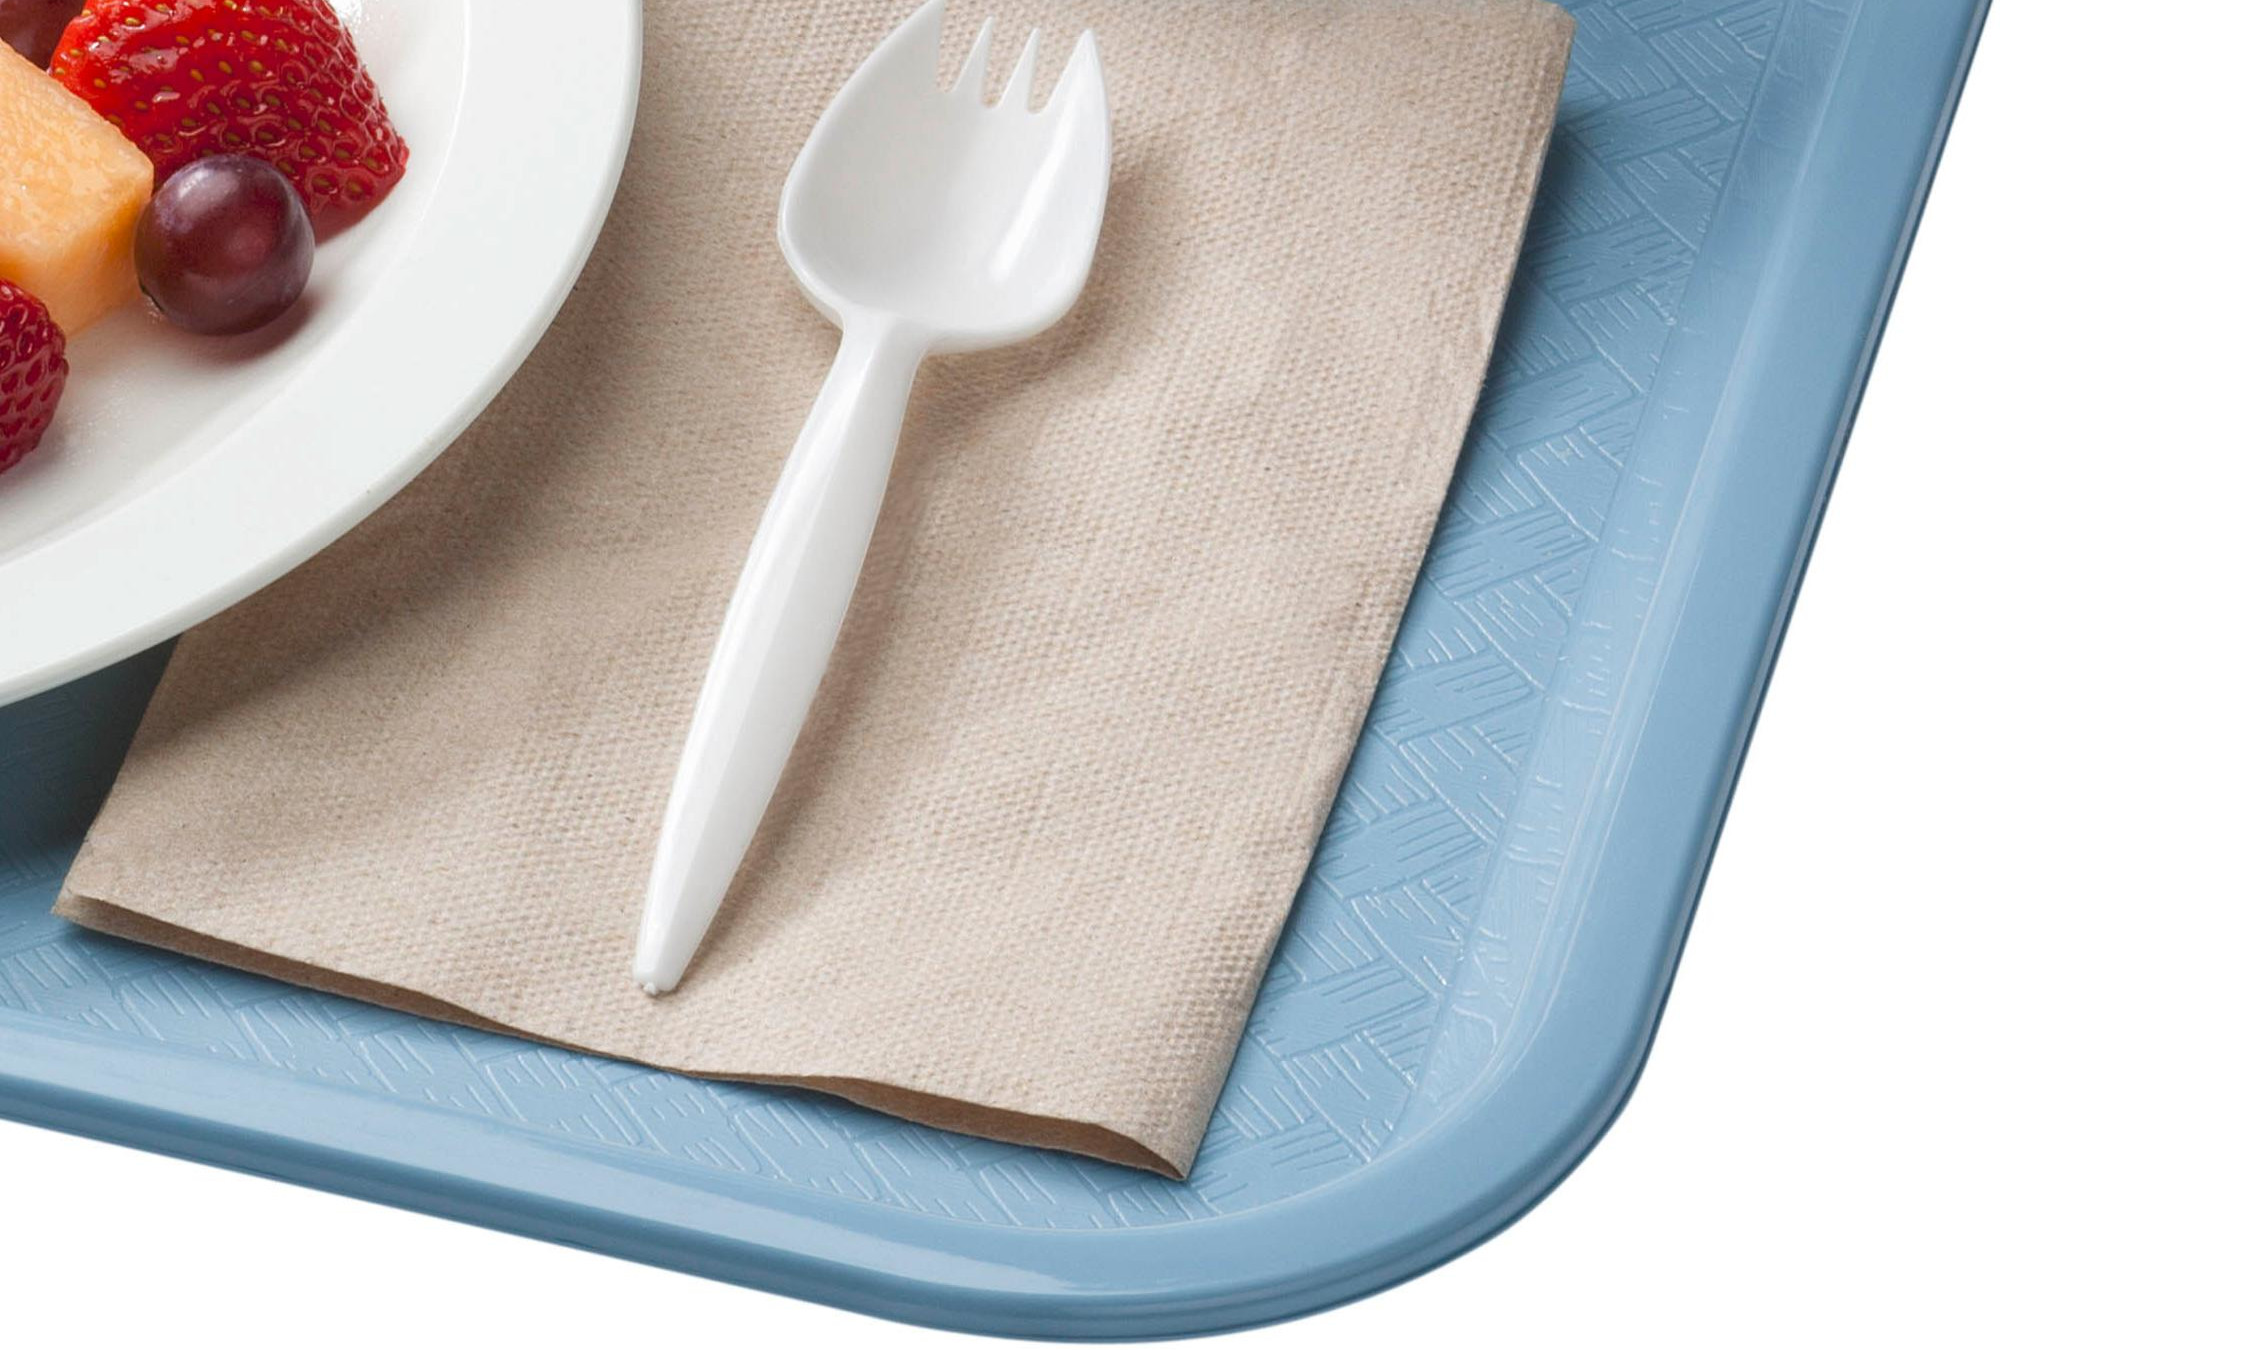
\includegraphics[width=\linewidth]{usda_spork.jpg}

\newpage
\myBiggerTitle{GPU Programming Challenges}

{\LARGE

\begin{itemize}
  \item SIMT-style parallelism: assign \myKeyA{similar work} to \myKeyA{different threads}
  \begin{itemize}
    \item e.g. parallel vector add: \texttt{y[threadIdx.x] += x[threadIdx.x]}
  \end{itemize}
  \item Specialization: assign \myKeyA{different work} to \myKeyA{different threads}
  \begin{itemize}
    \item e.g. overlap data movement work and compute work
  \end{itemize}
  \item Synchronization between threads
  \begin{itemize}
    \item Avoid unexpected long stalls
    \item ...don't make a mistake
  \end{itemize}
\end{itemize}

\myKeyA{Overall theme:} overlap work predictably (without introducing subtle bugs)
}

\newpage
{\LARGE
\begin{itemize}
\item A1
\item A2
\item A3
\item A4
\item A5
\item A6
\item A7
\item A8
\item A9
\item A10
\end{itemize}

}

\end{document}
